\section{Methodology}\label{sec:chp6:method}

Our \ac{mpmri} \ac{cad} system consists of 7 different steps: pre-processing, segmentation, registration, feature detection, balancing, feature selection/extraction, and finally classification.
%% It should be noted that \ac{cad} system designed deals with multiparametric \ac{mri} data. 

\subsection{Pre-processing}\label{subsec:chp6:method:PP}

\begin{figure}
  \hspace*{\fill}
  \subfigure[]{\label{fig:adcpdf1}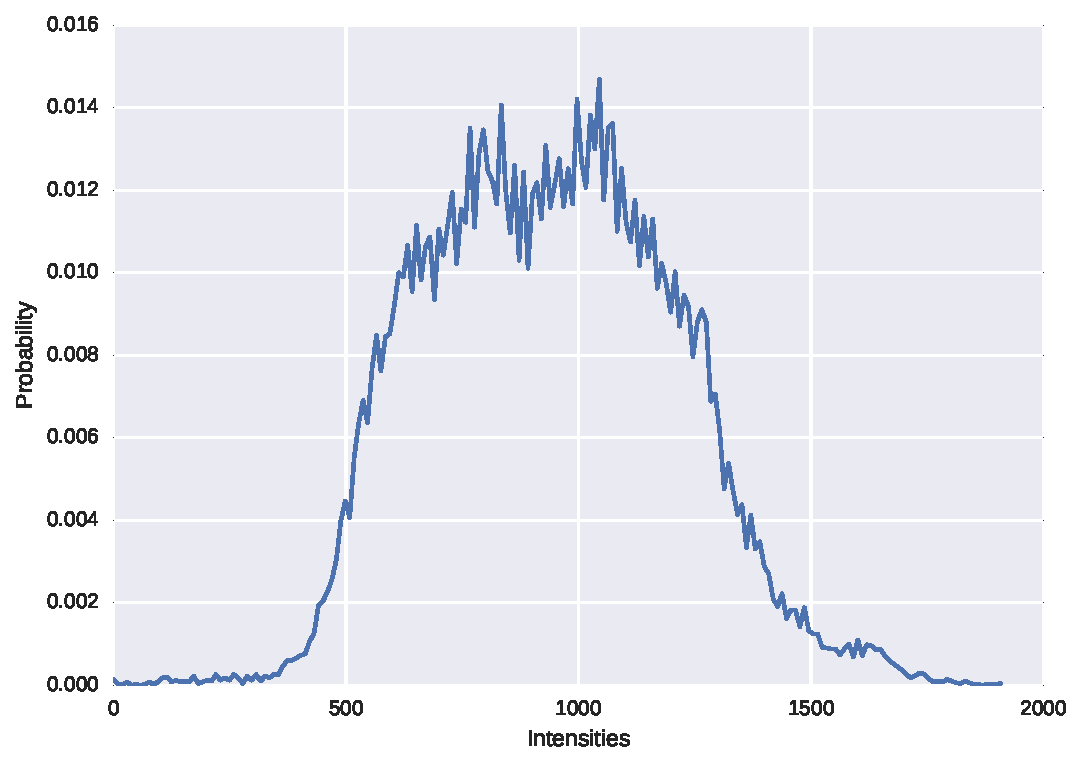
\includegraphics[width=.3\textwidth]{6_pipeline/figures/adc_pdf.pdf}}
  \hfill
  \subfigure[]{\label{fig:adcpdf2}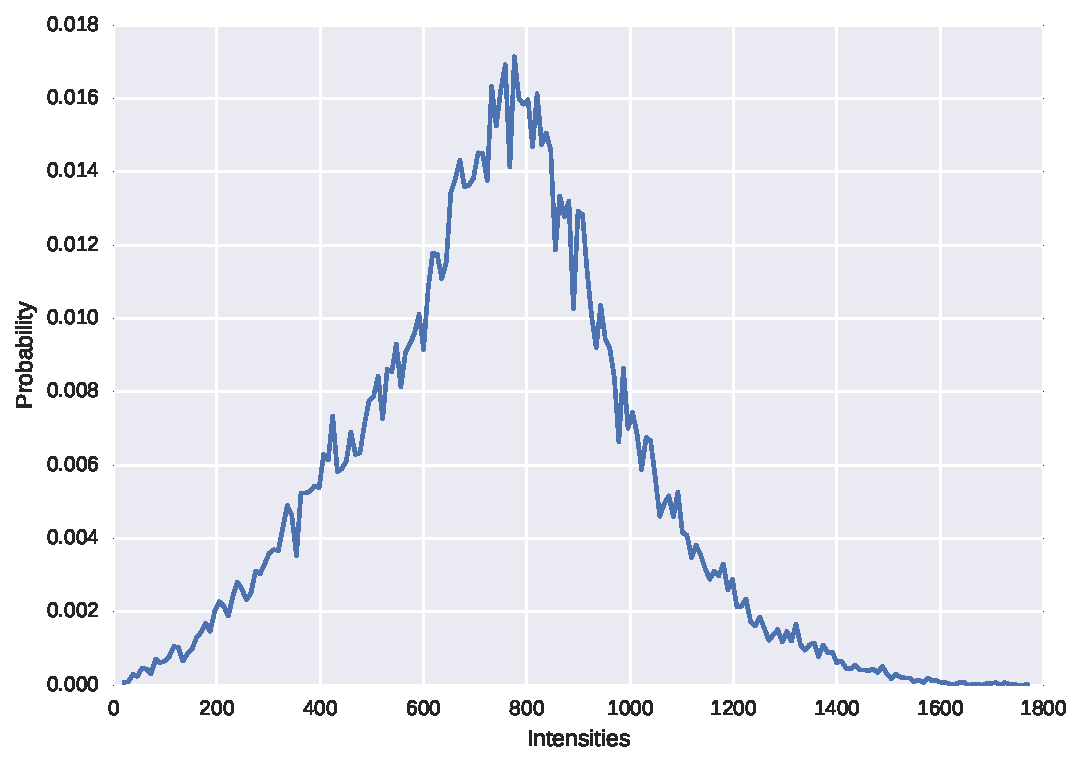
\includegraphics[width=.3\textwidth]{6_pipeline/figures/adc_pdf_2.pdf}}
  \hfill
  \subfigure[]{\label{fig:adcpdf3}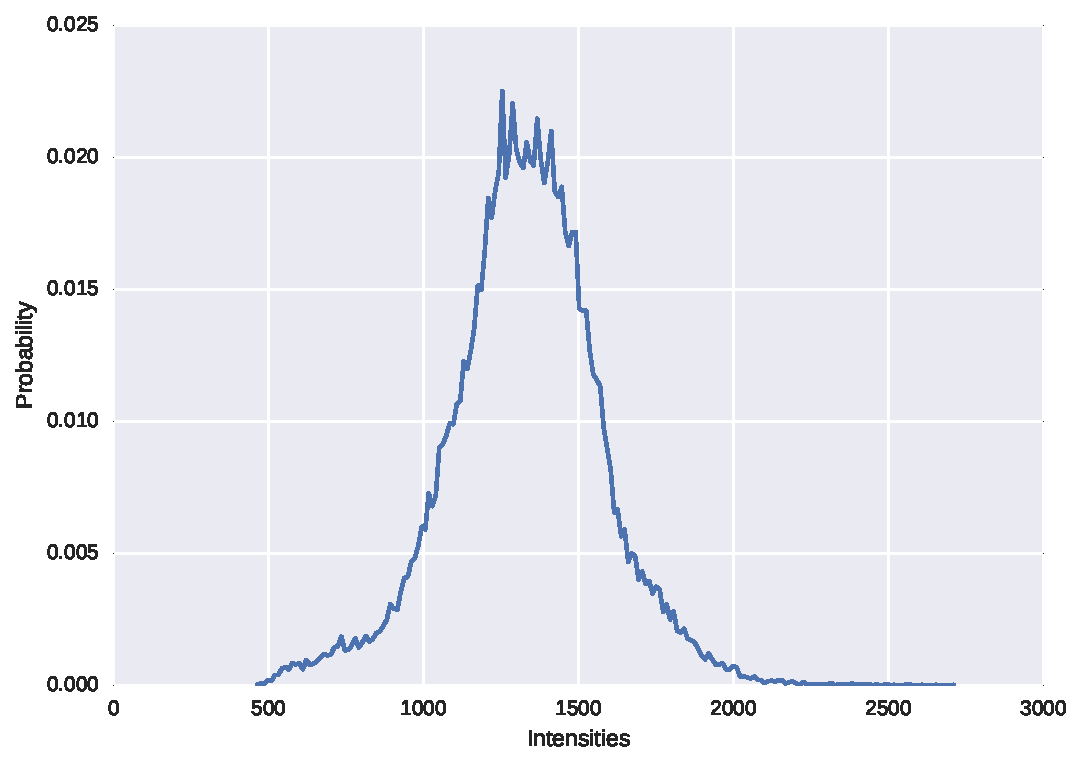
\includegraphics[width=.3\textwidth]{6_pipeline/figures/adc_pdf_3.pdf}}
  \hspace*{\fill}
  \caption[Illustration of the \acs*{pdf} of the \acs*{adc} coefficient within the prostate.]{Illustration of the variability of the \acs*{pdf} of the \acs*{adc} coefficient within the prostate for 3 patients.}
  \label{fig:adcpdf}
\end{figure}


The reader can refer to \acs{sec}\,\ref{subsec:chp3img-reg:prepro} to have an extensive overview of the state-of-the-art methods used to pre-process \ac{mpmri} data.
Three types of pre-processing are used for \ac{mri} images: (i) noise filtering, (ii) bias correction, and (iii) standardization/normalization.
Our dataset is based on \SI{3}{\tesla} images without endorectal coil and therefore, the two first types of correction have not been considered as necessary.
Normalization is, however, a crucial step to reduce the inter-patient variations which allows to improve the learning during the classification stage.
\Ac{chp}~\ref{chap:5} presented two normalization methods to pre-process \ac{t2w}-\ac{mri} and \ac{dce}-\ac{mri}, respectively.
Therefore, we used these methods to standardize these images.
Regarding the \ac{adc} map normalization, the \ac{pdf} within the prostate does not follow a known distribution as depicted in \acs{fig}\,\ref{fig:adcpdf}.
Thus, one cannot use a parametric model to normalize these images and a non-parametric piecewise-linear normalization~\cite{Nyul2000} is the best option for this case.

Additionally, the \ac{mrsi} modality requires a specific pre-processing based on signal processing rather than image processing.
Therefore, the \ac{mrsi} modality has been pre-process to correct the phase, baseline, and frequency.
Regarding the problem of phase correction and frequency alignment, we use the most efficient method of the state-of-the-art review in \acs{sec}\,\ref{subsec:chp3img-reg:prepro}.
Indeed, as \citeauthor{Parfait2012} and \citeauthor{trigui2017automatic}~\cite{Parfait2012,trigui2016classification,trigui2017automatic}, the phase of each \ac{mrsi} spectra is corrected using the approach of \citeauthor{Chen2002}~\cite{Chen2002}.
Along the same line, the frequency shift of each spectra is corrected by aligning to \SI{4.65}{\ppm} the maximum of an inferred function fitted to the residuals of water, using a Voigt profile as in \acs{eq}\,\eqref{eq:voigt}.

\begin{equation}
  V(x; \sigma, \gamma) = \frac{\mathbf{R} \left[ w(z) \right]}{\sigma \sqrt{2\pi}} \ ,
  \label{eq:voigt}
\end{equation}

\noindent where $\mathbf{R} \left[ w(z) \right]$ is the real part of the Faddeva function for $z = \frac{x + i \gamma}{\sigma \sqrt{2}}$.

By assessing the qualitative results obtained in~\cite{Parfait2010}, the baseline correction method used by \citeauthor{Parfait2012} and \citeauthor{trigui2017automatic} does not provide an optimal solution for that matter.
The iterative low-pass filter enforce to much the smoothness of the baseline.
\citeauthor{xi2008baseline} propose a baseline detection derived from a parametric smoothing model~\cite{xi2008baseline}.
The \ac{nmr} signal is formalized as a sum of a pure signal, the baseline function, and an additive Gaussian noise such as:

\begin{equation}
  y_i = b_i + \mu_i e^{n_i} + \varepsilon_i
  \label{eq:methodBaselineDetectionModel}
\end{equation}

\noindent where $y_i$ is the \ac{nmr} signal, $b_i$ is the baseline, $\mu_i$ is the true signal, and $n_i$ and $\varepsilon_i$ are Gaussian noises.

\citeauthor{xi2008baseline} propose to find the baseline function

Xi et al. built the cost function presented in equation \ref{eq:methodBaselineDetectionCostFunction} based on the assumption of the model chosen (equation \ref{eq:methodBaselineDetectionModel}) and that the baseline estimated should be smooth without being necessarily flat (figure \ref{fig:methodBaselineDetection2}) and that should be laid on the middle of the data in segments where there is only noise (figure \ref{fig:methodBaselineDetection3}) \cite{Xi2008}.

\begin{equation}
  F(b) = \sum_i b_i - A \sum_i (b_{i+1} + b_{i-1} - 2 b_i)^2 - B \sum_i (b_i - \gamma_i)^2 g(b_i - \gamma_i)
  \label{eq:methodBaselineDetectionCostFunction}
\end{equation}
where $g(\bullet)$ is the Heaviside function.

The cost function $F(b)$ is composed of three main terms:

\begin{itemize}
  \item $\sum_i b_i$ is the sum of all baseline points.
    \item $- A \sum_i (b_{i+1} + b_{i-1} - 2 b_i)^2$ is the smoothness penalty. This term tends to be small for linear segments while it will be large for small curvature radii.
      \item $- B \sum_i (b_i - \gamma_i)^2 g(b_i - \gamma_i)$ is the negative penalty. This term tends to be nonzero when the baseline is above the data point.
\end{itemize}

In order to compute the optimal baseline, the first term has to be maximized subject to both second and third terms (equation \ref{eq:methodBaselineDetectionMaxim}). 

\begin{equation}
  b_0 = \text{arg}\, \max F(\textbf{b})
  \label{eq:methodBaselineDetectionMaxim}
\end{equation}

At this stage, the two parameter $A$ and $B$ have to be chosen. Xi et al. have shown that the theoritical values are as in equation \ref{eq:methodBaselineDetectionParametersA} and \ref{eq:methodBaselineDetectionParametersB}.

\begin{equation}
  A = \frac{5 \times 10^{-9} n^4}{\sigma}
  \label{eq:methodBaselineDetectionParametersA}
\end{equation}
\begin{equation}
  B = \frac{1.25}{\sigma}
  \label{eq:methodBaselineDetectionParametersB}
\end{equation}
where $\sigma$ is an estimation of the standard deviation of the noise and $n$ is the total number of data point.

Hence, an estimation of the standard deviation of the noise of the spectrum has to be performed. In order to estimate this parameter, Xi et al. proposed to divide the spectrum into smaller sections and compute the variance and mean intensity for each region. Then, they proposed to use the LOWESS regression to fit a model to the variance versus mean intensity signal. Finally, the estimation of the standard deviation of the noise is the square root of the variance at zero mean intensity in the LOWESS regression (equation \ref{eq:methodBaselineDetectionNoise}).

\begin{equation}
  \sigma = \sqrt{\sigma^2_\varepsilon}
  \label{eq:methodBaselineDetectionNoise}
\end{equation}
where $\sigma^2_\varepsilon$ is the variance at zero mean intensity inferred using the LOWESS regression.

Once that all parameters are found, $\frac{\partial F(\textbf{b})}{\partial \textbf{b}} = 0$ has to be solved in order to maximize the function $F(\textbf{b})$ \cite{Xi2008}.

\subsection{Segmentation and registration}\label{subsec:chp6:method:Seg-Reg}

For this study, no segmentation method has been developed and the manual segmentation given by our radiologist has been used.
The prostate is suffering, however, from a misalignment between the different \ac{mri} modalities.
Therefore, three registrations have been developed to: (i) the patient motion during the \ac{dce}-\ac{mri} acquisition, (ii) the patient motion between the \ac{t2w}-\ac{mri} and the \ac{dce}-\ac{mri} acquisitions, and (iii) the patient motion between the \ac{t2w}-\ac{mri} and the \ac{adc} map acquisition.
All registrations are implemented in C++ using \ac{itk}.

The \ac{dce}-\ac{mri} acquisition being dynamic, some intra-patient might occur during the acquisition.
For each serie of this dynamic acquisition, each 3D volume is registered to the first volume acquired, to remove the residual motion.
The appearance in the \ac{dce}-\ac{mri} images, however, varies due to the presence or not of the contrast media.
Therefore, the metric chosen to be minimized is the \ac{mi} and the geometric transform has been set to a rigid transform.
The optimization is performed using a regular step gradient descent.

Once the intra-patient motions corrected, a registration to correct the alignment between the \ac{t2w}-\ac{mri} and the \ac{dce}-\ac{mri} acquisitions is performed.
For that matter, the prostate has been segmented in both modalities --- \ac{t2w}-\ac{mri} and \ac{dce}-\ac{mri} --- to create two binary masks.
Therefore, these 3D binary masks are directly registered using the \ac{mse} metric.
Unlike the previous registration, we use a more complex geometric transform by successively finding a rigid transformation, a coarse elastic transformation, and a fine elastic transformation.
B-splines transformation is used as the elastic transform.
These successive transformations allow to get a good initialization for the next transformation.
The transformation is inferred by minimizing the cost function using a regular step gradient descent.

The \ac{t2w}-\ac{mri} and \ac{adc} map acquisitions are identically registered than the the \ac{t2w}-\ac{mri} and the \ac{dce}-\ac{mri} modalities.
Additionally, the \ac{cap}, \ac{pz}, and \ac{cg} are segmented on the \ac{t2w}-\ac{mri} and thus the latter modality is used as the reference modality.

\subsection{Feature detection}\label{subsec:chp6:method:fea-det}




As presented in Sect.~\ref{subsec:chp3:img-clas:CADX-fea-dec}, variety of features have been extracted depending on each modality.
In this work we extract image, \ac{dce}, and \ac{mrsi}-based features from \ac{t2w}-\ac{mri} and \ac{adc}-\ac{mri} images, \ac{dce}-\ac{mri}, and \ac{mrsi}-signals respectively.

Voxel-wise texture, edge, and position-based 3-dimensional features are detected as image-based features.
Laplacian, Prewitt, Sobel, Kirsch operators as well as {\color{red} shaar} and Gabor filter bank are detected as edge-based features.
These features were extensively discussed in Sect.~\ref{subsec:chp3:img-clas:CADX-fea-dec}.
\ac{dct}, \ac{glcm} and \ac{lbp} features are detected as part of texture-based features.

All the \ac{dce}-features presented in Sect.~\ref{subsubsec:chp3:img-clas:CADX-fea-dec:DCE-fea} are extracted from \ac{dce}-\ac{mri} modality.
Whole-spectra, semi-quantitative and quantitative features were explained in details in Chapter.~\ref{chap:5}, Sect.~\ref{subsubsec:chp5:DCE-norm:stateart}.

\ac{mrsi}-based features were previously explained in Sect.~\ref{subsubsec:chp3:img-clas:CADX-fea-dec:MRSI-fea}. 
Whole sepctra and quantification features are extracted from \ac{mrsi}-modality.
  
\subsection{Feature balancing}\label{subsec:chp6:method:fea-bal}
Data imbalanced is a common problem while classifiying medical data.
Considering a binary classification problem, there is always a class (often the class indicating cancer, or disease patients) that have smallest number of samples (i.e, minority class) in comparison to the other class (i.e, majority class).
The problem of data balancing corresponds to equalize the number of samples of both the minority and majority classes.
This task can be achieved in either data or feature space while performing over-sampling of minority samples or under-sampling of majority samples.
In this section we compare different under and over-sampling techniques applied in feature space.

\subsubsection{\Acl*{us1}}
Techniques that reduce the number of samples of the majority class to be equal to the number of samples of minority class are referred as \ac{us1} techniques.
%Considering the problem of imbalanced, \ac{us} is performed such that the number of samples of the majority class is reduced to be equal to the number of samples of the minority class.
The following methods are considered to perform such balancing.

\begin{description}
  \item[\Ac{rus}] is performed by randomly selecting without replacement a subset of samples from the majority class such that the number of samples is then equal in both minority and majority classes.
  \item[\Ac{nm}] offers three different methods to under-sample the majority class~\cite{mani2003knn}.
In \ac{nm1}, samples from the majority class are selected such that for each sample, the average distance to the $k$ \ac{nn} samples from the minority class is minimum.
\ac{nm2} diverges from \ac{nm1} by considering the $k$ farthest neighbours samples from the minority class.
In \ac{nm3}, a subset $M$ containing samples from the majority class is generated by finding the $m$ \ac{nn} from each sample of the minority class.
Then, samples from the subset $M$ are selected such that for each sample, the average distance to the $k$ \ac{nn} samples from the minority class is maximum.
In our experiment, $k$ and $m$ are fixed to 3.
\item[\Ac{iht}]~\cite{smith2014instance} undersamples the samples which have a high hardness threshold.
Hardness indicates the likelihood of missclassification rate for each samples.
The notation of instance hardness are drawn through the decomposition of $p(h \vert t)$ using Bayes' theorem, where $h$ represent the mapping function used to mapp input features to their corresponding labels and $t$ represents the training set.
\begin{equation}
  IH_h(\langle x_{i}, y_{i}\rangle) = 1 - p(y_i \vert x_i, h).\
\label{eq:iht}
\end{equation}
The undersampling is performed by keeping the most probable samples (i.e, filtering the samples with high hardness value) through \ac{kcv} training sets while considering specific threshold for filtering.
%% The hardness of an instance is depedent on the instances in the training data and the algorithm used to produced h (h is a function mapping input features to their corresponding label , i.e, the classifier, or base learner function).

 
\end{description}

\subsubsection{\Acl*{os}}
Contratry to \ac{us1} techniques, the data balancing can be performed by \ac{os} in which the new samples belonging to the minority class are generated aiming at equalizing the number of samples in both classes.
The following methods are compared for \ac{os} techniques.
\begin{description}
\item[\Ac{ros}] is performed by randomly replicating the samples of the minority class such that the number of samples is equal in both minority and majority classes.
\item[\Ac{smote}] is a method to generate synthetic samples in the feature space~\cite{chawla2002smote}.
Let define $x_i$ as a sample belonging to the minority class.
Let define $x_{nn}$ as a randomly selected sample from the $k$ \ac{nn} of $x_i$, with $k$ set to 3.
Therefore, a new sample $x_j$ is generated such that $x_j = x_i + \sigma \left( x_{nn} - x_i \right)$, where $\sigma$ is a random number in the interval $\left[0,1\right]$.
\item[\Ac{smoteb1}]~\cite{han2005borderline} over samples the minority samples similar to \ac{smote}.
However, instead of usig all the minority samples, it focuses on the borderline samples of minority class.
Borderline samples simply indicate the samples that are closer to the other class.
In this method first the borderline samples of minority class are detected.
The sample, $x_{i}$ belongs to borderline samples if more than half of its $k$ \ac{nn} samples belong to majority class.
Synthetic data is then created based on \ac{smote} method for borderline samples and selection of their $s$ \ac{nn} from the minority class.
 
\item[\Ac{smoteb2}]~\cite{han2005borderline} performs similar to \ac{smoteb1}.
However, instead of generating synthetic samples from borderline samples and their $s$ \ac{nn} from the minority class, it also generate samples based on their \ac{nn} of majority samples.
Synthetic samples created based on majority samples are placed closer to samples of minority class.
\end{description}

\subsection{Feature selection and extraction}\label{subsec:chp6:method:fea-sel}
Different feature selection and extraction methods were presented in Sect.~\ref{subsec:chp3:img-clas:CADX-fea-ext}.
Among those \ac{pca} is used as feature extraction on  \ac{mrsi} and \ac{dce}-based features.
In addition to \ac{pca}, sparse-\ac{pca} and \ac{ica} are also used to extract distinct features from \ac{mrsi} and \ac{dce}-based features.

Similar to \ac{pca}, \ac{ica}~\cite{comon1994independent} is looking for independent components of the datat.
However, it does not require orthogonolaity of the space and does not assume Gaussian distribution for each independent source.
Therefore, opposit to \ac{pca} it can recover uniquely the signals themselve rather than  linear subspace in which the signals lie \cite{murphy2012machine}.

Sparse-\ac{pca}~\cite{zou2006sparse} is another approach for feaure extraction and dimension reduction.
Similar to \ac{pca}, this apprcoach project the data into linear combination of input data.
However, instaed of using original data, it uses the sparse representation of the data, and therefore projects them as linear combination of few input components rather than all of them.
Refereing to Eq.~\eqref{eq:eigpca}, the objective of sparse-\ac{pca} is formulated as maximizing the variance while maintinaing the sparse constraint:

\begin{eqnarray}
 && \argmax \quad   \mathbf{v}^{-1} \Sigma \mathbf{v}\ , \label{eq:sparsepca}\\ 
 && \text{subject to }  \Vert \mathbf{v} \Vert_{2} = 1\ , \nonumber \\
 && \Vert \mathbf{v} \Vert_{0} \leq k\ . \nonumber
\end{eqnarray}
\noindent where $k$ indicates that number of non-zero elements in $\mathbf{v}$.

ANOVA F-test and \ac{rf} are used as feature selection approaches for image-based features.
ANOVA F-test can assess the superiority or inferiority of the features 
ANOVA F-test evaluates the potential of one feature at a time to predict the target label by measuring between group variability over within group variability.
This test finds which features on average are superior of inferior to others versus the null hypothesis.
%% \begin{equation}
%% F = \frac{}{}
%% \label{eq:Ftest}
%% \end{equation} 


\subsection{Classification}\label{subsec:chp6:method:clas}
Variety of classifiers were explained in Sect.~\ref{subsec:chp3:img-clas:CADX-clas}. 
Among those \ac{rf} is used as ensemble approach while classifying inidiviual modalities, where as a meta classifier using stacking of \ac{rf} is used for combination of different modalities.

Staking~\cite{wolpert1992stacked} is a way to create a meta classifier using different base learners.
This method uses the prediction of different base learners as input for a meta leaner and combines them into a final decision.
Each base learner is trained on the training set and its prediction on the validation set is fet to the meta learner.
The test sample, in a similar way is first classified by the base learners and their prediction is passed through the meta learner in order to achieve the final decision.

 
